\documentclass{article}
\title{Implementazione di un modulo per il calcolo del Determinante in una Libreria Ibrida Cpu-Gpu}
\author{Povero Toninus}

\usepackage[cm]{fullpage}%set dei margini

\usepackage{xcolor} %pacchetto per cambiare il colore di simboli nei display math
\usepackage{graphicx}

\usepackage{amsmath}  %http://tex.stackexchange.com/questions/40028/highlight-elements-in-the-matrix
\usepackage{tikz}
\usetikzlibrary{arrows,matrix,positioning}

\usepackage[utf8x]{inputenc}%gli accenti

\usepackage{verbatim}%per i commenti
\usepackage{hyperref}% per i link a file

\definecolor{redi}{RGB}{255,38,0}
\definecolor{redii}{RGB}{200,50,30}
\definecolor{yellowi}{RGB}{255,251,0}
\definecolor{bluei}{RGB}{0,150,255}
\definecolor{blueii}{RGB}{135,247,210}
\definecolor{blueiii}{RGB}{91,205,250}
\definecolor{blueiv}{RGB}{115,244,253}
\definecolor{bluev}{RGB}{1,58,215}
\definecolor{orangei}{RGB}{240,143,50}
\definecolor{yellowii}{RGB}{222,247,100}
\definecolor{greeni}{RGB}{166,247,166}


\tikzset{ 
table/.style={
  matrix of nodes,
  row sep=-\pgflinewidth,
  column sep=-\pgflinewidth,
  nodes={rectangle,draw=black,text width=1.25ex,align=center},
  text depth=0.25ex,
  text height=1ex,
  nodes in empty cells
  },
texto/.style={font=\footnotesize\sffamily},
title/.style={font=\small\sffamily}
}


\newcommand\CellText[2]{%
  \node[texto,left=of mat#1,anchor=east]
  at (mat#1.west)
  {#2};
}

\newcommand\SlText[2]{%
  \node[texto,left=of mat#1,anchor=west,rotate=75]
  at ([xshift=3ex]mat#1.north)
  {#2};
}

\newcommand\RowTitle[2]{%
\node[title,left=6.3cm of mat#1,anchor=west]
  at (mat#1.north west)
  {#2};
}


\begin{document}


\begin{displaymath}
\left[ \begin{array}{ccc} a_{00} & a_{01} & a_{02} \\ a_{10} & a_{11} & a_{12} \\ a_{20} & a_{21} & a_{22}  \end{array} \right] 
\mapsto
\left[ \begin{array}{cc} \color{blue}b_{00} & \color{blue}b_{01} \\ \color{blue}b_{10} & \color{blue}b_{11}  \end{array} \right] 
\mapsto
\left[ \begin{array}{c} \color{green}D   \end{array} \right] 
\end{displaymath}










Condensazione di Salem Said
\begin{displaymath}
b_{i,j} =
\left| \begin{array}{cc} a_{0,l} & a_{0,j+1}  \\ a_{i+1 , l} & a_{i+1 , j+1}  \end{array} \right| 
\end{displaymath}

\begin{displaymath}
	\left[ \begin{array}{ccccc} 
		\cdots & a_{0j} & \cdots & \color{red}a_{0l} & \cdots  \\ 
		 & \vdots &  & \vdots &  \\ 
		\cdots & \color{blue}a_{ij} & \cdots & a_{il}  & \\
		& \vdots &  & \vdots & \ddots
	\end{array} \right] 
\end{displaymath}

    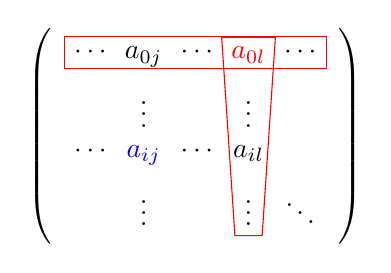
\begin{tikzpicture}
        \matrix [matrix of math nodes,left delimiter=(,right delimiter=)] (m)
        {
            \cdots & a_{0j} & \cdots & \color{red}a_{0l} &\cdots \\
            		 & \vdots &  & \vdots &  \\ 
			\cdots & \color{blue}a_{ij} & \cdots & a_{il}  & \\
			& \vdots &  & \vdots & \ddots \\
        };  
       \draw[color=red] (m-1-1.north west) -- (m-1-5.north east) -- (m-1-5.south east) -- (m-1-1.south west) -- (m-1-1.north west);
       \draw[color=red] (m-1-4.north west) -- (m-1-4.north east) -- (m-4-4.south east) -- (m-4-4.south west) -- (m-1-4.north west);
    \end{tikzpicture}











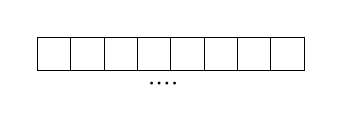
\begin{tikzpicture}[node distance =0pt and 0.5cm]

\matrix[table] (mat1) 
{
 & & & & & & & \\
};



\matrix[below=of mat1] (mat2) 
{
$\cdot$ &$\cdot$ &$\cdot$ &$\cdot$    \\
};

 
\end{tikzpicture}\newpage


\begin{tikzpicture}[node distance =0pt and 0.5cm]

\matrix[matrix of math nodes] (matThread) 
{
\cdot & \cdot & \cdot & \cdot & & & & \\
};

\matrix[table,below=of m] (matGlobal) 
{
  & & & & & & & & &\\
};

\matrix[table,below=of matGlobal] (matShared) 
{
 & & &  \\
};

\matrix[table,below=of matShared] (matresult) 
{
 & |[fill=redi]| \\
};



\draw[color=red] (matThread-1-1.north west) -- (matThread-1-2.north east) -- (matThread-1-2.south east) -- (matThread-1-1.south west) -- (matThread-1-1.north west);
\draw[color=red] (matThread-1-3.north west) -- (matThread-1-4.north east) -- (matThread-1-4.south east) -- (matThread-1-3.south west) -- (matThread-1-3.north west);

\draw[color=red] (matGlobal-1-1.north west) -- (matGlobal-1-2.north east) -- (matGlobal-1-2.south east) -- (matGlobal-1-1.south west) -- (matGlobal-1-1.north west);
\draw[color=red] (matThread-1-3.north west) -- (matThread-1-4.north east) -- (matThread-1-4.south east) -- (matThread-1-3.south west) -- (matThread-1-3.north west);
 
\end{tikzpicture}

\end{document}